\subsection{Application Architecture}
\label{sec:application_architecture}
While the application is only designed as proof of concept, the structure of it is not random. Given that it acts as an example implementation, it is designed to demonstrate how the server functionality can be used for an application. The game is coded as an Android application. As many other types of software, there is different versions of Android, and when deciding which version to target, one should usually consider that anyone using older versions will be excluded from using the application. Given that the developed application is not meant for release, this concern has been disregarded. As such the application is developed for a somewhat newer version of Android called "Jelly bean" (Version 4.1 or alternatively API level 16). This version was announced on June 27th, 2012\cite{jelly-bean}. This potentially allows for easier programming as a newer version can mean both additional features and bugfixes.

The application is built using standard Android activities. These activities represent one screen layout each - For example a login screen or a lobby screen for a game.\cite{android-activity} The exact coupling and flow of these activities can be seen in figure \ref{fig:appstructure}. The idea is that after login, the user has a menu from where the application branches out, providing the option to create, join or resume a game. What is not shown in the figure is that the user can still use the Android "back" button. This will always lead back to the Menu screen, allowing the user to pick something else to do. Using the button from the Menu logs the user out to the login screen, and from here it will exit the application.

\begin{figure}[H]
\centering
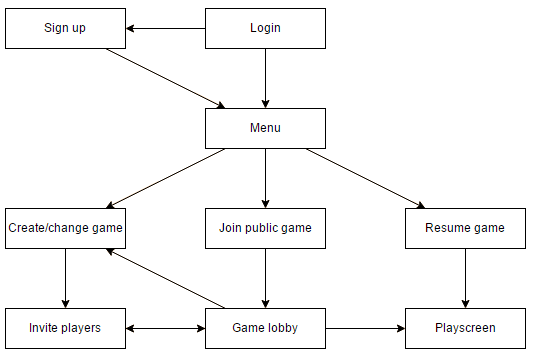
\includegraphics[width=\textwidth]{billeder/appstructure.png}
\caption{Structure of the application}
\label{fig:appstructure}
\end{figure}

\subsection{Coupling with server functionality}
\label{subsec:server-coupling}
With the exception of the Menu, all activities require communication with the server. To facilitate this easily, three classes are used, namely \textit{Client}, \textit{EncodeServerXML} and \textit{DecodeServerXML}. These are described in the paragraphs below. For a visualization of the structure in which they are used, see figure \ref{fig:appcommunication}.

\paragraph{Client}
The client class is responsible for all communication with the server. The implementation is very simple. It connects to the server upon being instantiated and is then able to send and receive strings using methods called \textit{send} and \textit{read}. For any desired server functionality, the programmer should use the send method. Given that the string sent is readable by the server, this will prompt the server to perform the requested action, and send a response to the client. To get this answer, the programmer should use the read method to retrieve the returned XML string.

\paragraph{EncodeServerXML and DecodeServerXML}
The server accepts some pre-defined XML strings to understand commands sent from the client. The reasoning behind this is described in section \ref{sec:interfaces}. For a programmer it could be tedious to write up XML strings in the different activities. To ease this process, a static class called EncodeServerXML was created which generates these strings for the programmer. By using this, it is enough to call a method on the class with the required parameters, for example \textit{EncodeServerXML.login} using username and password as arguments. This exact usage can be seen in figure \ref{fig:facadepattern}. Similar to EncodeServerXML, DecodeServerXML handles XML returned from the server. The server responds in the same kind of XML that it receives. To ease the parsing of these XML strings, a static method has been designed to read these responses and convert any important information to usable types of data.

\begin{figure}[H]
\centering
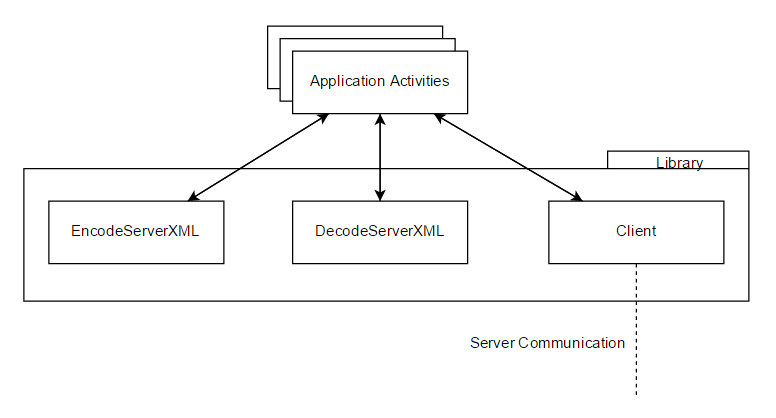
\includegraphics[width=\textwidth]{billeder/appcommunication.png}
\caption{Abstraction of server communication}
\label{fig:appcommunication}
\end{figure}